\section{Betriebssysteme}

\begin{defi}{Betriebssystem}
    Das \emph{Betriebssystem} liegt als Softwareschicht zwischen dem Rechner bzw. der \\ \emph{Software-Hardwareschnittstelle}, die das BIOS zur Verfügung stellt, und den Anwenderprogrammen.
    Das heißt, dass ein Endnutzer nur mit dem Betriebssystem, den vom Betriebssystem bereitgestellten Dienstprogrammen und den Anwenderprogrammen in Kontakt kommt.

    \begin{center}
        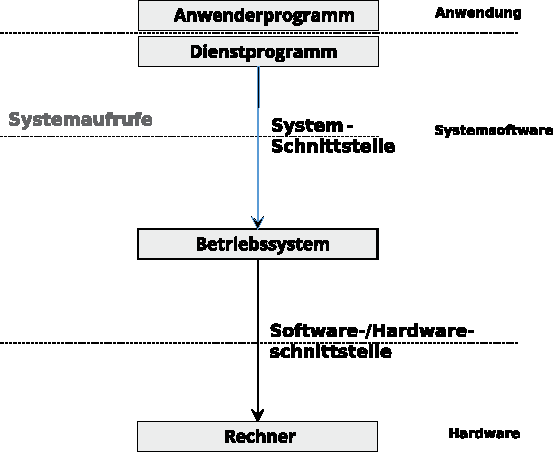
\includegraphics[]{images/betriebssysteme.pdf}
    \end{center}
\end{defi}

\begin{bonus}{Anforderungen an ein Betriebssystem}
    \begin{itemize}
        \item Hohe Zuverlässigkeit und Leistung
        \item Einfache Bedienbarkeit und Wartbarkeit
        \item Niedrige Kosten
    \end{itemize}
\end{bonus}

\begin{bonus}{Batchsysteme}
    \emph{Batchsysteme} sind dazu gedacht, Rechenaufgaben ohne Nutzereingabe abzuarbeiten.
    Dazu gibt es eine \emph{Job Queue}, in welche Aufgaben eingestellt werden.
    Diese Aufgaben werden dann bearbeitet und die Ergebnisse an den Nutzer ausgegeben.
\end{bonus}

\begin{bonus}{Dialogsysteme}
    \emph{Dialogsysteme} sind auf eine Interaktion mit dem Benutzer ausgelegt.
    Sie sind die wohl geläufigste Form von Betriebssystemen, da diese Form auf z.B. Desktop-Computern eingesetzt wird.

    Dialogsysteme werden noch einmal unterteilt in \emph{Single User}- und \emph{Multi-User-Systeme}.
\end{bonus}

\begin{bonus}{Echtzeitsysteme}
    \emph{Echtzeitsysteme} sind reaktive Systeme, die mit Hilfe von Sensoren Ereignisse registrieren und anhand von Aktoren darauf reagieren.
    Dabei ist die zeitliche Abfolge bzw. die Dauer der Ausführung von Interesse.
\end{bonus}

\subsection{Prozess}

\begin{defi}{Prozess}
    Ein \emph{Prozess} ist die Abstraktion eines in Ausführung befindelichen Programms.

    Er besteht aus den \emph{Programmbefehlen} und dem \emph{Prozesskontext}.

    Der \emph{Prozesskontext} besteht aus dem privaten Adressraum des Prozessors, geöffneten Streams und abhängigen Prozessen.
\end{defi}

\begin{defi}{Prozesszustände}
    \begin{center}
        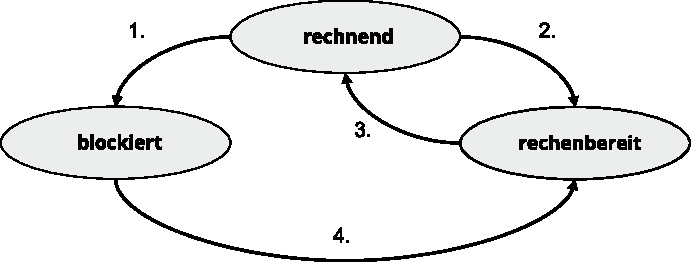
\includegraphics[]{images/prozesszustaende.pdf}
    \end{center}
    \begin{enumerate}
        \item Der Prozess muss auf ein externes Ereignis warten.
        \item Die Zeitscheibe des Prozesses ist abgelaufen, oder ein höher priorisierter Prozess muss ausgeführt werden.
        \item Der Prozess bekommt eine neue Zeitscheibe zugeteilt.
        \item Das externe Ereignis, auf das der Prozess gewartet hat, ist eingetreten.
    \end{enumerate}
\end{defi}

\begin{bonus}{Multitasking}
    \textbf{Preemptives Multitasking}:
    \begin{itemize}
        \item Betriebssystem entscheidet, wann welcher Prozess zur Ausführung kommt
        \item Benutzer erhält Eindruck von Parallelität
    \end{itemize}

    \textbf{Kooperatives Multitasking}:
    \begin{itemize}
        \item Prozess bestimmt selbst, wann er den Prozessor abgibt
        \item \emph{Nachteile}
              \subitem - z.B. Endlosschleifen können das gesamte System zum Absturz bringen
              \subitem - das Betriebssystem kann nicht berechnen, wann der Prozessor wieder frei ist
    \end{itemize}
\end{bonus}

\begin{defi}{Scheduling}
    Die Zuteilung von Zeitscheiben wird \emph{Scheduling} genannt und ist der Kern der Prozessverwaltung.
    Das Scheduling sollte dabei jederzeit die folgenden Eigenschaften erfüllen:
    \begin{itemize}
        \item \emph{Fairness}: Jeder Prozess erhält einen gerechten Anteil der CPU-Zeit.
        \item \emph{Effizienz}: Die CPU und andere Ressourcen sind möglichst vollständig ausgelastet.
    \end{itemize}
\end{defi}

\begin{bonus}{Priorität}
    \textbf{Statische Priorität}:
    \begin{itemize}
        \item Jeder Prozess erhält beim Start eine \emph{feste Priorität}
        \item Prozess mit \emph{höchster Priorität} bekommt als nächstes eine Zeitscheibe zugeteilt
        \item Oft in Echtzeitsystemen verwendet
    \end{itemize}

    \textbf{Dynamische Priorität}:
    \begin{itemize}
        \item Jeder Prozess erhält beim Start eine \emph{Anfangspriorität}
        \item Prozess mit \emph{höchster Priorität} bekommt als nächstes eine Zeitscheibe zugeteilt
        \item Prioritäten der Prozesse werden \emph{dynamisch geändert}
    \end{itemize}
\end{bonus}

\begin{algo}{Scheduling: FIFO (First In First Out)}
    Prozesse werden nach \emph{Reihenfolge} ihres Einfügens in die \emph{Job-Queue} bearbeitet.
    \begin{itemize}
        \item Zuteilung der CPU findet nur statt, wenn laufender Prozess wartet oder sich beendet
        \item Jeder Prozess kommt garantiert an die Reihe
        \item Kurze Prozesse müssen unter Umständen sehr lange warten, bis sie ausgeführt werden
    \end{itemize}
\end{algo}

\begin{algo}{Scheduling: SJF (Shortest Job First)}
    Prozesse werden aufsteigend nach ihrer \emph{geschätzten Ausführungszeit} bearbeitet.
    \begin{itemize}
        \item Große Prozesse kommen möglicherweise nie an die Reihe, wenn stets kleinere dazukommen
        \item Wartezeit auf das Ergebnis eines Prozesses sich in etwa proportional zur Ausführungszeit
    \end{itemize}
\end{algo}

\begin{algo}{Scheduling: MLFQ (Multilevel Feedback Queue)}
    Bei diesem Ansatz gibt \emph{mehrere FIFO-Queues}, denen jeweils
    eine \emph{Priorität} zugeordnet ist.

    Ein neuer Prozess wird immer in der Queue mit
    \emph{höchster Priorität} eingeordnet.

    Wird der Prozess während der ersten Zeitscheibe fertig,
    so verlässt er das System.

    Gibt er die CPU freiwillig ab, beispielsweise weil er
    durch das Warten auf ein externes Ereignis blockiert wird, wird er, sobald er wieder
    bereit ist, in \emph{dieselbe Queue wieder einsortiert} und dort weiter ausgeführt.

    Verbraucht der Prozess seine Zeitscheibe vollständig, so wird er in die \emph{nächst-niedriger priorisierte FIFO-Queue} eingereiht. Dort gelten wieder dieselben Regeln wie vorher.

    Verbraucht der Prozess immer weiter seine Zeitscheiben vollständig, kommt er
    schließich in der \emph{am niedrigsten priorisierten Queue} an.
    Dort verweilt er, bis er abgearbeitet wurde, d.h. es gibt \emph{keine Möglichkeit} wieder in höher priorisierte Queues
    eingestuft zu werden.

    Wieviele FIFO-Queues es gibt, ist vom konkreten Einsatzszenario abhängig.
\end{algo}

\begin{bonus}{Mittlere Verweildauer}
	Scheduling Strategien lassen sich im konkreten Anwendungsfall anhand der \emph{mittleren Verweildauer} der Prozesse in der Job-Queue vergleichen. Ordnet man eine Liste mit $n$ Prozessen und ihren Bearbeitungszeiten $t_1, \ldots , t_n$ entsprechend der gewählten Scheduling Strategie an, so terminieren diese zu den Zeitpunkten $T_1 = t_1, T_2 = T_1 + t_2, \ldots , T_n = T_{n-1} + t_n$. Dabei sind $T_1, \ldots , T_n$ die Verweildauern der Prozesse. Die mittlere Verweildauer ist also:
	$$
		\frac{T_1 + T_2 + \ldots + T_n}{n}
	$$
\end{bonus}

\subsection{Speicherverwaltung}

\begin{defi}{Reale Speicherverwaltung}
    Jedem Prozess wird ein zusammenhängener Block im Hauptspeicher zugeteilt.
    Wird in diesem Kontext der Arbeitsspeicher direkt aus den Prozessen heraus adressiert, spricht man von \emph{realer Speicherverwaltung}.

    Das bedeutet auch, dass die Größe des physikalisch vorhandenen Hauptspeichers die Anzahl der gleichzeitig ausführbaren Prozesse begrenzt.

    \emph{Nachteile}:
    \begin{itemize}
        \item Es muss Platz für das \emph{gesamte Programm und die Daten} gefunden werden.
        \item Es kannt nicht mehr Speicher genutzt werden, als \emph{physikalisch vorhanden}.
        \item Anforderung, zusammenhängender Speicherblöcke zu finden, verschärft Problem der \emph{Fragmentierung}.
    \end{itemize}
\end{defi}

\begin{bonus}{Fragmentierung}
    \emph{Fragmentierung} passiert dann, wenn mehrere, kleine Blöcke im Hauptspeicher frei sind und unter der Prämisse, dass einem
    Prozess ein zusammenhängender Block im Hauptspeicher zugeordnet werden
    muss, dies eventuell zu einer Situation führt, in der kein neuer Prozess gestartet
    werden kann, obwohl in Summe genügend Hauptspeicher frei wäre.
\end{bonus}

\begin{defi}{Swapping}
    Beim \emph{Swapping} wird der
    Hauptspeicherinhalt eines Prozesses auf den \emph{Hintergrundspeicher}, beispielsweise
    eine Festplatte (HDD), \emph{ausgelagert}, um Platz für andere Prozesse zu schaffen.

    Bekommt dann der Prozess, dessen Daten gerade auf dem Hintergrundspeicher liegen,
    die CPU zugeteilt, müssen seine Daten \emph{erneut in den Hauptspeicher geladen werden},
    wahrscheinlich nachdem die Daten eines anderen Prozesses ausgelagert wurden.
\end{defi}

\begin{defi}{Virtuelle Speicherverwaltung}
    Jedem Prozess wird ein \emph{scheinbar zusammenhängender Speicherbereich} zur Verfügung gestellt.
    Tatsächlich besteht der Speicher des Prozesses aus nicht zwangsläufig zusammenhängenden \emph{virtuelle Pages}.

    Der Prozess kann seinen Speicher mit \emph{virtuellen Adressen} beginnend bei 0 adressieren.

    Die Gesamtheit aller virtuellen Adressen wird als \emph{virtueller Adressraum} bezeichnet.
\end{defi}

\begin{defi}{Virtuelle Pages}
    \emph{Virtuelle Pages} werden auf Blöcke im Hauptspeicher gleicher Größe abgebildet.

    Hier kann auch \emph{Swapping} genutzt werden. In diesem Fall aber für einzelne Pages, nicht für den gesamten Hauptspeicherinhalt des Prozessors.
\end{defi}

\begin{defi}{Pagetable}
    Beim Zugriff auf eine virtuelle Speicheradresse durch einen Prozess muss diese
    Adresse in eine physikalische Adresse umgewandelt werden. Das geschieht anhand
    der \emph{Pagetable}, die das Betriebssystem \emph{für jeden Prozess} erstellt und aktualisiert.

    Da
    die Pagetable virtuelle Pages auf physikalische Pages gleicher Größe abbildet, gibt es einen Teil der Adresse, der sogenannte \emph{Offset}, der die Position der Daten innerhalb
    der Page angibt.

    Abhängig von
    der Größe der Pages besteht das Offset aus $m$ Bits.
    Für eine Pagegröße von 1MB
    werden beispielsweise 20 Bits als Offset benötigt.

    Der Rest der Adresse, die Seitennummer,
    muss dann anhand der Pagetable in die Basisadresse umgesetzt werden,
    um die Adresse im physikalischen Speicher zu erhalten. Da die Seitennummer aus
    $n$ Bits besteht, kann die Pagetable maximal $2^n$ Einträge enthalten.
\end{defi}

\begin{example}{Pagetable}
    Die Länge einer Adresse sei 16 Bit, aufgeteilt in je 8 Bit für Offset und Seitennummer.

    Es sei außerdem folgende Seitentabelle gegeben:

    \begin{center}
        \begin{tabular}{|c|c|c|}
            \hline
            \textbf{Eintrag} & \textbf{Gültig} & \textbf{Basisadresse} \\
            \hline
            00               & Nein            & -                     \\
            01               & Ja              & 0x17                  \\
            02               & Ja              & 0x20                  \\
            03               & Ja              & 0x08                  \\
            04               & Nein            & -                     \\
            05               & Ja              & 0x10                  \\
            \hline
        \end{tabular}
    \end{center}

    Dann können virtuelle Adressen anhand dieser Pagetable wie folgt umgesetzt werden:

    \begin{center}
        \begin{tabular}{|c|c|}
            \hline
            \textbf{virtuelle Adresse} & \textbf{physikalische Adresse}      \\
            \hline
            0x083A                     & ungültig (Seite 8 existiert nicht)  \\
            0x01FF                     & 0x17FF (Seite 1, Basisadresse 0x17) \\
            0x0505                     & 0x1005 (Seite 5, Basisadresse 0x10) \\
            0x043A                     & ungültig (Seite 4 ungültig)         \\
            \hline
        \end{tabular}
    \end{center}

    \emph{Hinweis}: Ist eine Adresse ungültig, wurde die dazugehörige Page in den Hintergrundspeicher ausgelagert. In diesem Fall muss die physikalische Page in den RAM geladen und die Pagetable aktualisiert werden.
\end{example}

\begin{bonus}{Paging on Demand}
    Das Vorgehen, aktuell
    unbenutzte Pages aus dem Hauptspeicher auf den Hintergrundspeicher auszulagern
    wird auch als \emph{Paging on Demand} bezeichnet.
    Das Ziel dabei ist, Arbeitsspeicher
    für andere Prozesse freizugeben.

    Dabei kann ein Prozess entweder Platz für eine
    bestimmte Anzahl von physikalischen Pages zugewiesen bekommen, die sich im
    Laufe der Prozessabarbeitung nicht ändert, oder es wird dynamisch anhand der aktuellen
    Speicherauslastung entschieden, wieviel Platz ein Prozess belegen darf.
\end{bonus}

\begin{algo}{Speicherverwaltung: FIFO (First In First Out)}
    Beim \emph{FIFO}-Verfahren wird
    diejenige Page ausgelagert, welche sich schon am längsten im Hauptspeicher
    befindet. Dazu muss in der Pagetable festgehalten werden, wann welche
    Page in den Hauptspeicher geladen wurde.
\end{algo}

\begin{algo}{Speicherverwaltung: LRU/LFU (Least Recently / Frequently Used)}
    Bei \emph{LRU}
    wird mitgehalten, wieviele Ladevorgänge seit der letzten Benutzung einer
    Page vorgenommen wurden. Das heißt, dass im Gegensatz zu FIFO, der
    Kontrollzustand bei der Verwendung einer Page wieder auf \glqq 0\grqq gesetzt wird.
\end{algo}

\begin{example}{Speicherverwaltung}
    Seitenanforderungen: 1, 2, 3, 4, 1, 2, 5, 1, 2, 3, 4, 5

    \textbf{FIFO-Strategie:}

    \begin{tabular}{|c|c|c|c|c|c|c|c|c|c|c|c|c|c|}
        \hline
        \multicolumn{1}{|c}{\textbf{Referenzfolge}} & \multicolumn{1}{c|}{} & 1                  & 2                  & 3                  & 4                  & 1                  & 2                  & 5                  & 1 & 2 & 3                  & 4                  & 5 \\
        \hline
        \hline
        \multirow{3}{*}{\textbf{Arbeitsspeicher}}   & Page 1                & \textcolor{red}{1} & 1                  & 1                  & \textcolor{red}{4} & 4                  & 4                  & \textcolor{red}{5} & 5 & 5 & 5                  & 5                  & 5 \\
                                                    & Page 2                &                    & \textcolor{red}{2} & 2                  & 2                  & \textcolor{red}{1} & 1                  & 1                  & 1 & 1 & \textcolor{red}{3} & 3                  & 3 \\
                                                    & Page 3                &                    &                    & \textcolor{red}{3} & 3                  & 3                  & \textcolor{red}{2} & 2                  & 2 & 2 & 2                  & \textcolor{red}{4} & 4 \\
        \hline
        \hline
        \multirow{3}{*}{\textbf{Kontrollzustand}}   & Page 1                & 0                  & 1                  & 2                  & 0                  & 1                  & 2                  & 0                  & 1 & 2 & 3                  & 4                  & 5 \\
                                                    & Page 2                & -                  & 0                  & 1                  & 2                  & 0                  & 1                  & 2                  & 3 & 4 & 0                  & 1                  & 2 \\
                                                    & Page 3                & -                  & -                  & 0                  & 1                  & 2                  & 0                  & 1                  & 2 & 3 & 4                  & 0                  & 1 \\
        \hline
    \end{tabular}

    9 Einlagerungen

    \textbf{LRU-Strategie:}

    \begin{tabular}{|c|c|c|c|c|c|c|c|c|c|c|c|c|c|}
        \hline
        \multicolumn{1}{|c}{\textbf{Referenzfolge}} & \multicolumn{1}{c|}{} & 1                  & 2                  & 3                  & 4                  & 1                  & 2                  & 5                  & 1 & 2 & 3                  & 4                  & 5                  \\
        \hline
        \hline
        \multirow{3}{*}{\textbf{Arbeitsspeicher}}   & Page 1                & \textcolor{red}{1} & 1                  & 1                  & \textcolor{red}{4} & 4                  & 4                  & \textcolor{red}{5} & 5 & 5 & \textcolor{red}{3} & 3                  & 3                  \\
                                                    & Page 2                &                    & \textcolor{red}{2} & 2                  & 2                  & \textcolor{red}{1} & 1                  & 1                  & 1 & 1 & 1                  & \textcolor{red}{4} & 4                  \\
                                                    & Page 3                &                    &                    & \textcolor{red}{3} & 3                  & 3                  & \textcolor{red}{2} & 2                  & 2 & 2 & 2                  & 2                  & \textcolor{red}{5} \\
        \hline
        \hline
        \multirow{3}{*}{\textbf{Kontrollzustand}}   & Page 1                & 0                  & 1                  & 2                  & 0                  & 1                  & 2                  & 0                  & 1 & 2 & 0                  & 1                  & 2                  \\
                                                    & Page 2                & -                  & 0                  & 1                  & 2                  & 0                  & 1                  & 2                  & 0 & 1 & 2                  & 0                  & 1                  \\
                                                    & Page 3                & -                  & -                  & 0                  & 1                  & 2                  & 0                  & 1                  & 2 & 0 & 1                  & 2                  & 0                  \\
        \hline
    \end{tabular}

    10 Einlagerungen
\end{example}

\newpage
\subsection{Dateisystemverwaltung}

\begin{defi}{BIOS (Basic Input/Output System)}
    Das \emph{BIOS}:
    \begin{itemize}
        \item ist die \emph{Firmware} bei x86-PCs
        \item liegt im \emph{nichtflüchtigen Speicher} auf der Hauptplatine des PCs
        \item leitet den \emph{Start} des \emph{Betriebssystems} ein
    \end{itemize}
\end{defi}

\begin{defi}{UEFI (Unified Extensible Firmware Interface)}
    \emph{UEFI} ist die zentrale Schnittstelle zwischen:
    \begin{itemize}
        \item der \emph{Firmware}
        \item den \emph{einzelnen Komponenten} eines Rechners
        \item und dem \emph{Betriebssystem}
    \end{itemize}
\end{defi}

\begin{bonus}{MBR (Master Boot Record)}
    Der \emph{MBR} besteht aus insgesamt 512 Byte, die sich auf 446 Byte
    für einen (optionalen) Bootloader, 64 Byte für die \emph{Partitionstabelle} und 2 Byte
    für eine \emph{} (0xAA55) aufteilen. Die Magic Number dient dazu, einen
    gültigen MBR zu identifizieren.

    In der Partitionstabelle können maximal 4 Partitionen
    definiert werden, d.h. die Festplatte kann in maximal 4 logische Einheiten aufgeteilt
    werden.
\end{bonus}

\begin{bonus}{GPT (GUID Partition Table)}
    Mit der Einführung von UEFI wurden auch die Limitierungen des
    MBR aufgehoben und die GPT als Nachfolger definiert.

    Die \emph{GPT} beinhaltet zu Beginn
    aus Kompatibilitätsgründen einen MBR, sodass ein hybrider Betrieb möglich
    ist. In der GPT können bis zu 128 Partitionen abgelegt werden.

    Zur Absicherung der
    GPT wird eine exakte Kopie der GPT am Ende des Datenträgers abgelegt.
\end{bonus}

\begin{defi}{Dateisystem}
    Ein Dateisystem ist im Prinzip eine Ablageorganisation für Daten auf einem Datenträger des Computers.
    Das Dateisystem muss sicherstellen,
    dass Dateien \emph{lesend und schreibend geöffnet} und auch wieder \emph{geschlossen} werden
    können. Das bedeutet, dass Dateinamen auf physikalische Adressen auf dem
    Datenträger abgebildet werden müssen.

    Spezielle Eigenschaften des Datenträgers
    (Festplatte, USB-Stick, ...) müssen berücksichtigt werden.

    Generell bieten
    alle (modernen) Dateisysteme folgende Attribute:
    \begin{itemize}
        \item Dateiname
        \item Ablageort (Ordner bzw. Verzeichnis)
        \item Dateigröße
        \item Zugriffsrecht
    \end{itemize}
\end{defi}

\begin{defi}{Lineare Dateisysteme}
    Bei linearen Dateisystemen werden Daten direkt hintereinander auf den Datenträger
    geschrieben. Das bedeutet, dass wahlfreier Zugriff nicht möglich ist. Daher finden
    diese Dateiysteme heutzutage nur noch Anwendung in Bereichen, in denen es nicht
    primär auf Geschwindigkeit ankommt.
\end{defi}

\begin{defi}{Hierarchische Dateisysteme}
    Daten werden auf hierarchischen Dateisystemen in einer Verzeichnisstruktur
    abgelegt.

    Diese Art von Dateisystem ist die wohl verbreiteste auf
    modernen Computern und kann auf Festplatten, SSDs, USB-Sticks, SD-Karten und
    sonstigen herkömmlichen Datenträgern verwendet werden.
\end{defi}

\begin{defi}{Netzwerkdateisysteme}
    In Netzwerkdateisystemen wird entfernter
    Speicher auf einem Server wie ein lokales Medium behandelt. Das Betriebssystem
    muss dann die Zugriffe auf Dateien in Netzwerkkommunikation umwandeln.
    Für den Nutzer
    eines Betriebsystems stellt sich Netzwerkspeicher allerdings in der Regel wie ein
    hierarchisches Dateisystem dar.
\end{defi}

\begin{bonus}{Sicherheitsaspekte}
    \textbf{Paralleler Zugriff im Multitasking}:
    \begin{itemize}
        \item Bereitstellung von Locks für den Dateizugriff
    \end{itemize}

    \textbf{Stromausfall während einer Schreiboperation}:
    \begin{itemize}
        \item Es muss Datenkonsistenz gewährleistet werden
        \item Atomare Operationen, welche entweder abgeschlossen oder ausstehend sind
              \subitem $\to$ Journalingdateisysteme
    \end{itemize}
\end{bonus}

\begin{defi}{Journalingdateisysteme}
    Bei einem Journalingdateisystem werden alle Aktionen auf der Festplatte protokolliert
    und erst als gültig aufgefasst, nachdem das Beenden der Aktion auf dem Dateisystem
    im \emph{Journal} (Protokoll) vermerkt wurde.

    \begin{itemize}
        \item \emph{Metadatenjournaling}:
              \subitem - Konsistenz des Dateisystems
        \item \emph{Fulljournaling}:
              \subitem - Konsistenz des Dateisystems
              \subitem - Konsistenz der Dateiinhalte
    \end{itemize}

\end{defi}
